\subsection*{Задача 5. Gibbs Sampler for Gamma-Poisson model}
\addcontentsline{toc}{section}{Задача 5. Gibbs Sampler for Gamma-Poisson model}

\setcounter{subsection}{5}
\setcounter{equation}{0}

Нехай задано Баєсову модель такого вигляду:
\begin{align}
    & X_{ij} \,|\, \theta_i \overset{\scalebox{0.5}{ind}}{\sim} \mathrm{Poiss}(\theta_i),\ i=\overline{1,n},\ j=\overline{1,m}, \label{task 5 - eq: Bayes model Xij} \\
    & \theta_i \,|\, \sigma \overset{\scalebox{0.5}{i.i.d.}}{\sim} \mathrm{Gamma}(k,\sigma),\ i=\overline{1,n}, \label{task 5 - eq: Bayes model theta} \\
    & \sigma^{-1} \sim \mathrm{Exp}(1), \label{task 5 - eq: Bayes model sigma}
\end{align}
при цьому $k$ є відомим. Іншими словами, для кожної згенерованої випадкової величини~$\sigma$ з експоненціального розподілу генерується значення~$\theta_i$ з Гамма-розподілу, і надалі~--- набір випадкових величин~$X_{i1},\ldots,X_{im}$ з розподілу Пуасона з параметром~$\theta_i$.

\subsubsection*{Завдання (a): Gibbs Sampler}
\addcontentsline{toc}{subsection}{Завдання (a): Gibbs Sampler}

Завдання полягає у тому, щоб навести повні викладки одного кроку вибірки Гіббса для генерування апостеріорних розподілів параметрів~$\theta_i$ та~$\sigma$. Однак, перш ніж переходити до алгоритму, наведемо явний вигляд розподілів, які розглядатимуться у подальших міркуваннях.  

Дискретна випадкова величина~$\xi$ має розподіл Пуасона з параметром~$\lambda$, якщо: 
\begin{equation}\label{task 5 - eq: dPoisson}
    \xi \sim \mathrm{Poiss}(\lambda) \ \Longleftrightarrow \ P(\xi=x) = \frac{\lambda^{x}e^{-\lambda}}{x!} 
\end{equation}

Неперервна випадкова величина~$\eta$ має Гамма-розподіл з <<shape parameter>> $k>0$ та <<scale parameter>>~$\sigma>0$, якщо:
\begin{equation}\label{task 5 - eq: dGamma}
    \eta \sim \mathrm{Gamma}(k,\sigma) \ \Longleftrightarrow \ f_{\eta}(x) = \frac{x^{k-1}}{\sigma^{k}\Gamma(k)}\, e^{-x/\sigma}\, \mathbbm{1}(x>0)
\end{equation}

Кажуть, що неперервна випадкова величина~$\eta^{-1}$ має обернений Гамма-розподіл з параметрами~$k>0$ та~$\sigma>0$, якщо:
\begin{equation}\label{task 5 - eq: dIG}
    \eta^{-1} \sim \mathrm{IG}(k,\sigma) \ \Longleftrightarrow \ f_{\eta^{-1}}(x) = \frac{x^{-k-1}}{\Gamma(k)}\,\sigma^{k} e^{-\sigma/x}\, \mathbbm{1}(x>0)
\end{equation}

Наостанок наведемо вигляд щільности експоненціального розподілу з параметром~$\lambda$ для неперервної випадкової величини $\zeta^{-1}:$
\begin{equation}\label{task 5 - eq: dExp}
    \zeta^{-1} \sim \mathrm{Exp}(\lambda) \ \Longleftrightarrow \ f_{\zeta^{-1}}(x) = \lambda e^{-\lambda x}\, \mathbbm{1}(x>0),
\end{equation}
при цьому випадкова величина $\zeta$ матиме щільність виду
\begin{equation}\label{task 5 - eq: dInvExp}
    f_{\zeta}(x) = \lambda x^{-2} e^{-\lambda/x}\, \mathbbm{1}(x>0)
\end{equation}

Тож нехай ініційовано пару значень~$\left( \sigma^{(0)};\theta_1^{(0)},\ldots,\theta_n^{(0)} \right)$. Тоді один крок вибірки Гіббса складатиметься із таких пунктів:
\begin{enumerate}
    \item Використовуючи значення~$\sigma^{(0)}$, згенерувати значення~$\theta_i^{(1)}$ з так званого <<full conditional distribution for parameter~$\theta_i$>>~--- $f(\theta_i \,|\, \sigma^{(0)}; X_{i1},\ldots,X_{im})$; 
    \item Маючи значення~$\theta_i^{(1)}$, згенерувати значення~$\sigma^{(1)}$ з <<full conditional distribution for parameter~$\sigma$>>~--- $f(\sigma \,|\, \theta_1^{(1)},\ldots,\theta_n^{(1)}; X_{11},\ldots,X_{1m};\ldots;X_{n1},\ldots,X_{nm})$; 
\end{enumerate}

Зауважимо, що повний умовний розподіл одного параметра пропорційний сумісному розроділу, в якому інший параметр вважається фіксованим. Продемонструємо це, застосувавши ланцюгове правило:
\begin{equation}\label{task 5 - eq: full theta conditional distribution}
    \underbracket{f(\theta_i, \sigma \,|\, X_{i1},\ldots,X_{im})}_{\text{сумісний розподіл}} = \underbracket{f(\theta_i \,|\, \sigma; X_{i1},\ldots,X_{im})}_{\text{повний умовний розподіл}} \underbracket{f(\sigma \,|\, X_{i1},\ldots,X_{im})}_{\text{не залежить від $\theta_i$}}
\end{equation}

Таким чином переконуємося, що повний умовний розподіл як фунція від~$\theta_i$ пропорційний сумісному розподілу, в якому значення~$\sigma$ покладено фіксованим. Аналогічним чином для параметра~$\sigma$:
\begin{equation}\label{task 5 - eq: full sigmaconditional distribution}
    \underbracket{f(\theta_i, \sigma \,|\, X_{i1},\ldots,X_{im})}_{\text{сумісний розподіл}} = \underbracket{f(\sigma \,|\, \theta_i; X_{i1},\ldots,X_{im})}_{\text{повний умовний розподіл}} \underbracket{f(\theta_i \,|\, X_{i1},\ldots,X_{im})}_{\text{не залежить від $\sigma$}}
\end{equation}

Отже, опишемо один крок вибірки Гіббса:
\begin{enumerate}
    \item Маючи~$\sigma^{(0)}$, згенеруємо значення~$\theta_i^{(1)}$ із відповідного умовного розподілу. Послідовно скористаємося такими викладками: щойно продемонтрованою властивістю~\eqref{task 5 - eq: full theta conditional distribution} у переході~(1), формулою Баєса у переході~(2), ланцюговим правилом у переході~(3) та незалежністю значень вибірки даних у кроці~(4):
        \begin{align*}\label{task 5 - eq: chain of rules under full conditional distribution}
            f(\theta_i \,|\, \sigma^{(0)}; X_{i1},\ldots,X_{im})
            & \overset{\scalebox{0.5}{(1)}}{\propto} f(\theta_i, \sigma^{(0)} \,|\, X_{i1},\ldots,X_{im}) \propto \\
            & \overset{\scalebox{0.5}{(2)}}{\propto} f(X_{i1},\ldots,X_{im} \,|\, \theta_i, \sigma^{(0)}) f(\theta_i, \sigma^{(0)}) = \\
            & \overset{\scalebox{0.5}{(3)}}{=} f(X_{i1},\ldots,X_{im} \,|\, \theta_i, \sigma^{(0)}) f(\theta_i \,|\, \sigma^{(0)}) f(\sigma^{(0)}) = \\
            & \overset{\scalebox{0.5}{(4)}}{=} \prod_{j=1}^{m} f(X_{ij} \,|\, \theta_i, \sigma^{(0)}) f(\theta_i \,|\, \sigma^{(0)}) f(\sigma^{(0)}) \stepcounter{equation}\tag{\theequation}
        \end{align*}

        З огляду на вигляд функцій щільностей заданої Баєсової моделі~\eqref{task 5 - eq: Bayes model Xij} --~\eqref{task 5 - eq: Bayes model sigma}, матимемо:
        \begin{align*}
            f(\theta_i \,|\, \sigma^{(0)}; X_{i1},\ldots,X_{im}) \propto \prod_{j=1}^{m} \frac{\theta_i^{X_{ij}} e^{-\theta_i}}{X_{ij}!} 
            & \times \frac{\theta_i^{k-1}}{\left[\sigma^{(0)}\right]^{k}\Gamma(k)}\, e^{-\theta_i/\sigma^{(0)}} \mathbbm{1}(\theta_i>0) \times \\
            & \times \left[\sigma^{(0)}\right]^{-2}e^{-1/\sigma^{(0)}} \mathbbm{1}(\sigma^{(0)}>0) \stepcounter{equation}\tag{\theequation}
        \end{align*}

        Відкидаючи множники, які не мають фунцкіональної залежності від~$\theta_i$, отримуємо такий вираз:
        \begin{align}
            f(\theta_i \,|\, \sigma^{(0)}; X_{i1},\ldots,X_{im}) \propto \theta_i^{m\overline{X}_i + k - 1}\, e^{-\theta_i(m + 1/\sigma^{(0)})}\, \mathbbm{1}(\theta_i>0)
        \end{align}

        А відтак, аналогічно до перетворень у формулі~\eqref{eq: theta posterior} з'ясовуємо вигляд апостеріорного розподілу параметра~$\theta_i:$
        \begin{equation}\label{task 5 - eq: posterior theta distribution}
            \theta_i \,|\, \sigma^{(0)}; X_{i1},\ldots,X_{im} \sim \mathrm{Gamma}\left( k+m\overline{X}_i,\frac{\sigma^{(0)}}{1+\sigma^{(0)}m} \right)
        \end{equation}

        Отже, використовуючи~$\sigma^{(0)}$, генеруємо значення~$\theta_i^{(1)}$ із розподілу~\eqref{task 5 - eq: posterior theta distribution}.

    \item Маючи~$\theta_i^{(1)}$, згенеруємо значення~$\sigma^{(1)}$ із відповідного повного умовного розподілу. В силу аналогічних кроків, як це показано для виведення формули~\eqref{task 5 - eq: chain of rules under full conditional distribution}, матимемо:
        \begin{multline*}
            f(\sigma \,|\, \theta_1^{(1)},\ldots,\theta_n^{(1)}; X_{11},\ldots,X_{1m};\ldots;X_{n1},\ldots,X_{nm}) \propto \\
            \propto f(X_{11},\ldots,X_{1m};\ldots;X_{n1},\ldots,X_{nm} \,|\, \theta_1^{(1)},\ldots,\theta_n^{(1)}; \sigma) f(\theta_1^{(1)},\ldots,\theta_n^{(1)} \,|\, \sigma) f(\sigma), \stepcounter{equation}\tag{\theequation}
        \end{multline*}
        а отже, зважаючи на незалежність випадкових величин $\theta_1^{(1)},\ldots,\theta_n^{(1)}$, отримаємо
        \begin{multline*}
            f(\sigma \,|\, \theta_1^{(1)},\ldots,\theta_n^{(1)}; X_{11},\ldots,X_{1m};\ldots;X_{n1},\ldots,X_{nm}) \propto \\
            \propto \prod_{i=1}^{n} f(X_{i1},\ldots,X_{im} \,|\, \theta_i^{(1)}, \sigma) \prod_{i=1}^{n} f(\theta_i^{(1)} \,|\, \sigma) f(\sigma), \stepcounter{equation}\tag{\theequation}
        \end{multline*}
        і як наслідок властивості вибірки даних:
        \begin{multline*}
            f(\sigma \,|\, \theta_1^{(1)},\ldots,\theta_n^{(1)}; X_{11},\ldots,X_{1m};\ldots;X_{n1},\ldots,X_{nm}) \propto \\
            \propto \prod_{i=1}^{n} \prod_{j=1}^{m} f(X_{ij} \,|\, \theta_i^{(1)}, \sigma) \prod_{i=1}^{n} f(\theta_i^{(1)} \,|\, \sigma) f(\sigma) \stepcounter{equation}\tag{\theequation}
        \end{multline*}

        Відтак, з огляду на вигляд функцій щільностей заданої Баєсової моделі, вираз розписуватиметься як:
        \begin{multline*}
            f(\sigma \,|\, \theta_1^{(1)},\ldots,\theta_n^{(1)}; X_{11},\ldots,X_{1m};\ldots;X_{n1},\ldots,X_{nm}) \propto \\
            \propto \prod_{i=1}^{n} \prod_{j=1}^{m} \frac{\left[ \theta_i^{(1)} \right]^{X_{ij}} e^{-\theta_i^{(1)}}}{X_{ij}!} \times \prod_{i=1}^{n} \frac{\left[ \theta_i^{(1)} \right]^{k-1}}{\sigma^{k}\Gamma(k)}\, e^{-\theta_i^{(1)}/\sigma} \mathbbm{1}(\theta_i^{(1)}>0) \times \\ 
            \times \sigma^{-2}e^{-1/\sigma} \mathbbm{1}(\sigma>0) \stepcounter{equation}\tag{\theequation}
        \end{multline*}
       
        Відкидаючи множники, які не мають фунцкіональної залежності від~$\sigma$, отримуємо такий вираз:
        \begin{multline*}
            f(\sigma \,|\, \theta_1^{(1)},\ldots,\theta_n^{(1)}; X_{11},\ldots,X_{1m};\ldots;X_{n1},\ldots,X_{nm}) \propto \\
            \propto \sigma^{-nk-2}\, e^{-(n\overline{\theta^{(1)}} + 1)/\sigma}\, \mathbbm{1}(\sigma>0) \stepcounter{equation}\tag{\theequation}
        \end{multline*}

        У виразі, наведеному вище, впізнаємо обернений Гамма-розподіл~\eqref{task 5 - eq: dIG}:
        \begin{equation}\label{task 5 - eq: posterior sigma distribution}
            \sigma \,|\, \theta_i^{(1)}; X_{11},\ldots,X_{nm} \sim \mathrm{IG}\left( nk+1, n\overline{\theta^{(1)}} + 1 \right)
        \end{equation}

        Отже, використовуючи набір~$\theta_i^{(1)}$, генеруємо значення~$\sigma^{(1)}$ із розподілу~\eqref{task 5 - eq: posterior sigma distribution}.
\end{enumerate}

\subsubsection*{Завдання (b): \texttt{R-base} Gibbs Sampler}
\addcontentsline{toc}{subsection}{Завдання (b): \texttt{R-base} Gibbs Sampler}

Виконаємо засобами мови \texttt{R} вибірку Гіббса згідно із викладками, наведеними у попередньому підрозділі. Вибірку даних~\eqref{task 5 - eq: Bayes model Xij} задамо з файлу \texttt{hw5.csv}. Покладемо~$n=k=3$ та $m=100$, тобто матимемо Баєсову модель вигляду
\begin{align}
    & X_{ij} \,|\, \theta_i \overset{\scalebox{0.5}{ind}}{\sim} \mathrm{Poiss}(\theta_i),\ i=\overline{1,3},\ j=\overline{1,100}, \\
    & \theta_i \,|\, \sigma \overset{\scalebox{0.5}{i.i.d.}}{\sim} \mathrm{Gamma}(3,\sigma),\ i=\overline{1,3}, \\
    & \sigma^{-1} \sim \mathrm{Exp}(1)
\end{align}

Тож параметрами вибірки слугуватимуть значення~$\sigma$ та вектор~$\left( \theta_1,\theta_2,\theta_3 \right)$. Поклавши початкове значення~$\sigma^{(0)}=1$, проведемо $100$ кроків для <<розгону>> алгоритму і фіксуватимемо наступні $N=10\,000$ кроків для визначення апостеріорного розподілу невідомих параметрів. 

Наведемо нижче основні програмні блоки. До прикладу, у Лістингу~\ref{code: update theta} продемонстровано функцію для оновлення параметрів~$(\theta_1,\theta_2,\theta_3)$.

\vspace{0.4cm}
\begin{lstlisting}[
    style           = myR,
    % backgroundcolor = {},
    caption         = {Крок оновлення вектора параметрів~$(\theta_1,\theta_2,\theta_3)$},
    label           = {code: update theta},
]
update_theta <- function(x, sigma, k, n, m) {
    theta_values <- array(dim = n)

    for (i in 1:n) {
        shape_theta <- k + m * mean(x[, i])
        scale_theta <- sigma / (1.0 + sigma * m)

        theta_values[i] <- rgamma(1, shape = shape_theta, scale = scale_theta)
    }

    return(theta_values)
}
\end{lstlisting}

\vspace{0.4cm}
Нижче у Лістингу~\ref{code: update sigma} продемонстровано програмну реаілізацію оновлення значення~$\sigma$.

\vspace{0.4cm}
\begin{lstlisting}[
    style           = myR,
    % backgroundcolor = {},
    caption         = {Крок оновлення параметра~$\sigma$},
    label           = {code: update sigma},
]
update_sigma <- function(x, theta, k, n, m) {
    shape_sigma <- n * k + 1
    scale_sigma <- n * mean(theta) + 1

    sigma_value <- 1 / rgamma(1, shape = shape_sigma, scale = 1 / scale_sigma)

    return(sigma_value)
}
\end{lstlisting}

\vspace{0.4cm}
Запуск основного алгоритму вибірки Гіббса (Лістинг~\ref{code: gibbs sampler}) показано нижче у Лістингу~\ref{code: run gibbs sampler}.

\vspace{0.4cm}
\begin{lstlisting}[
    style           = myR, 
    % backgroundcolor = {},
    caption         = {Імплементація алгоритму вибірки Гіббса},
    label           = {code: gibbs sampler},
]
gibbs <- function(data, n_iter, init, prior, n, m) {
    # Initialize arrays to store variables
    sigma_out <- array(dim = c(n_iter, 1))
    theta_out <- array(dim = c(n_iter, 3))

    sigma_now <- init$sigma

    # Gibbs sampler
    for (i in 1:n_iter) {
        theta_now <- update_theta(
            x = data, sigma = sigma_now, k = prior$k, n = n, m = m
        )
        sigma_now <- update_sigma(
            x = data, theta = theta_now, k = prior$k, n = n, m = m
        )

        theta_out[i, ] <- theta_now
        sigma_out[i, ] <- sigma_now
    }

    cbind(sigma = sigma_out[, 1], theta1 = theta_out[, 1], theta2 = theta_out[, 2], theta3 = theta_out[, 3])
}
\end{lstlisting}

\vspace{0.4cm}
\begin{lstlisting}[
    style           = myR, 
    % backgroundcolor = {},
    caption         = {Запуск вибірки Гіббса},
    label           = {code: run gibbs sampler},
]
# Load the dataset
x <- read.csv("hw5.csv")

# Set main parameters
n <- ncol(x)
m <- nrow(x)

prior <- list()
prior$k <- 3

init <- list()
init$sigma <- 1.0

set.seed(53)
posterior <- gibbs(
    data = x,
    n_iter = 10e3 + 100,
    init = init,
    prior = prior,
    n = n,
    m = m
)

# Exclude first 100 iterations (burn-in period)
posterior <- tail(posterior, -100)
\end{lstlisting}

\vspace{0.4cm}
На Рис.~\ref{pic: Gibbs Sampler traceplot} продемонстровано результати: <<trace plot>> отриманого ланцюга Маркова та апостеріорний розподіл параметрів~$\sigma$ та $\theta_1$. Перш ніж перейти до подальших висновків, проведемо огляд автоколеляції утвореного ланцюга. Автоколеляція як така вказує на міру лінійної залежності (в межах~$[-1,1]$) поточного значення відносно попередніх значень (lags). З Рис.~\ref{pic: Gibbs Sampler autocorrelation} бачимо, що автокореляція значень практично відсутня.  

\vspace{0.4cm}
\begin{figure}[H]\centering
    \center{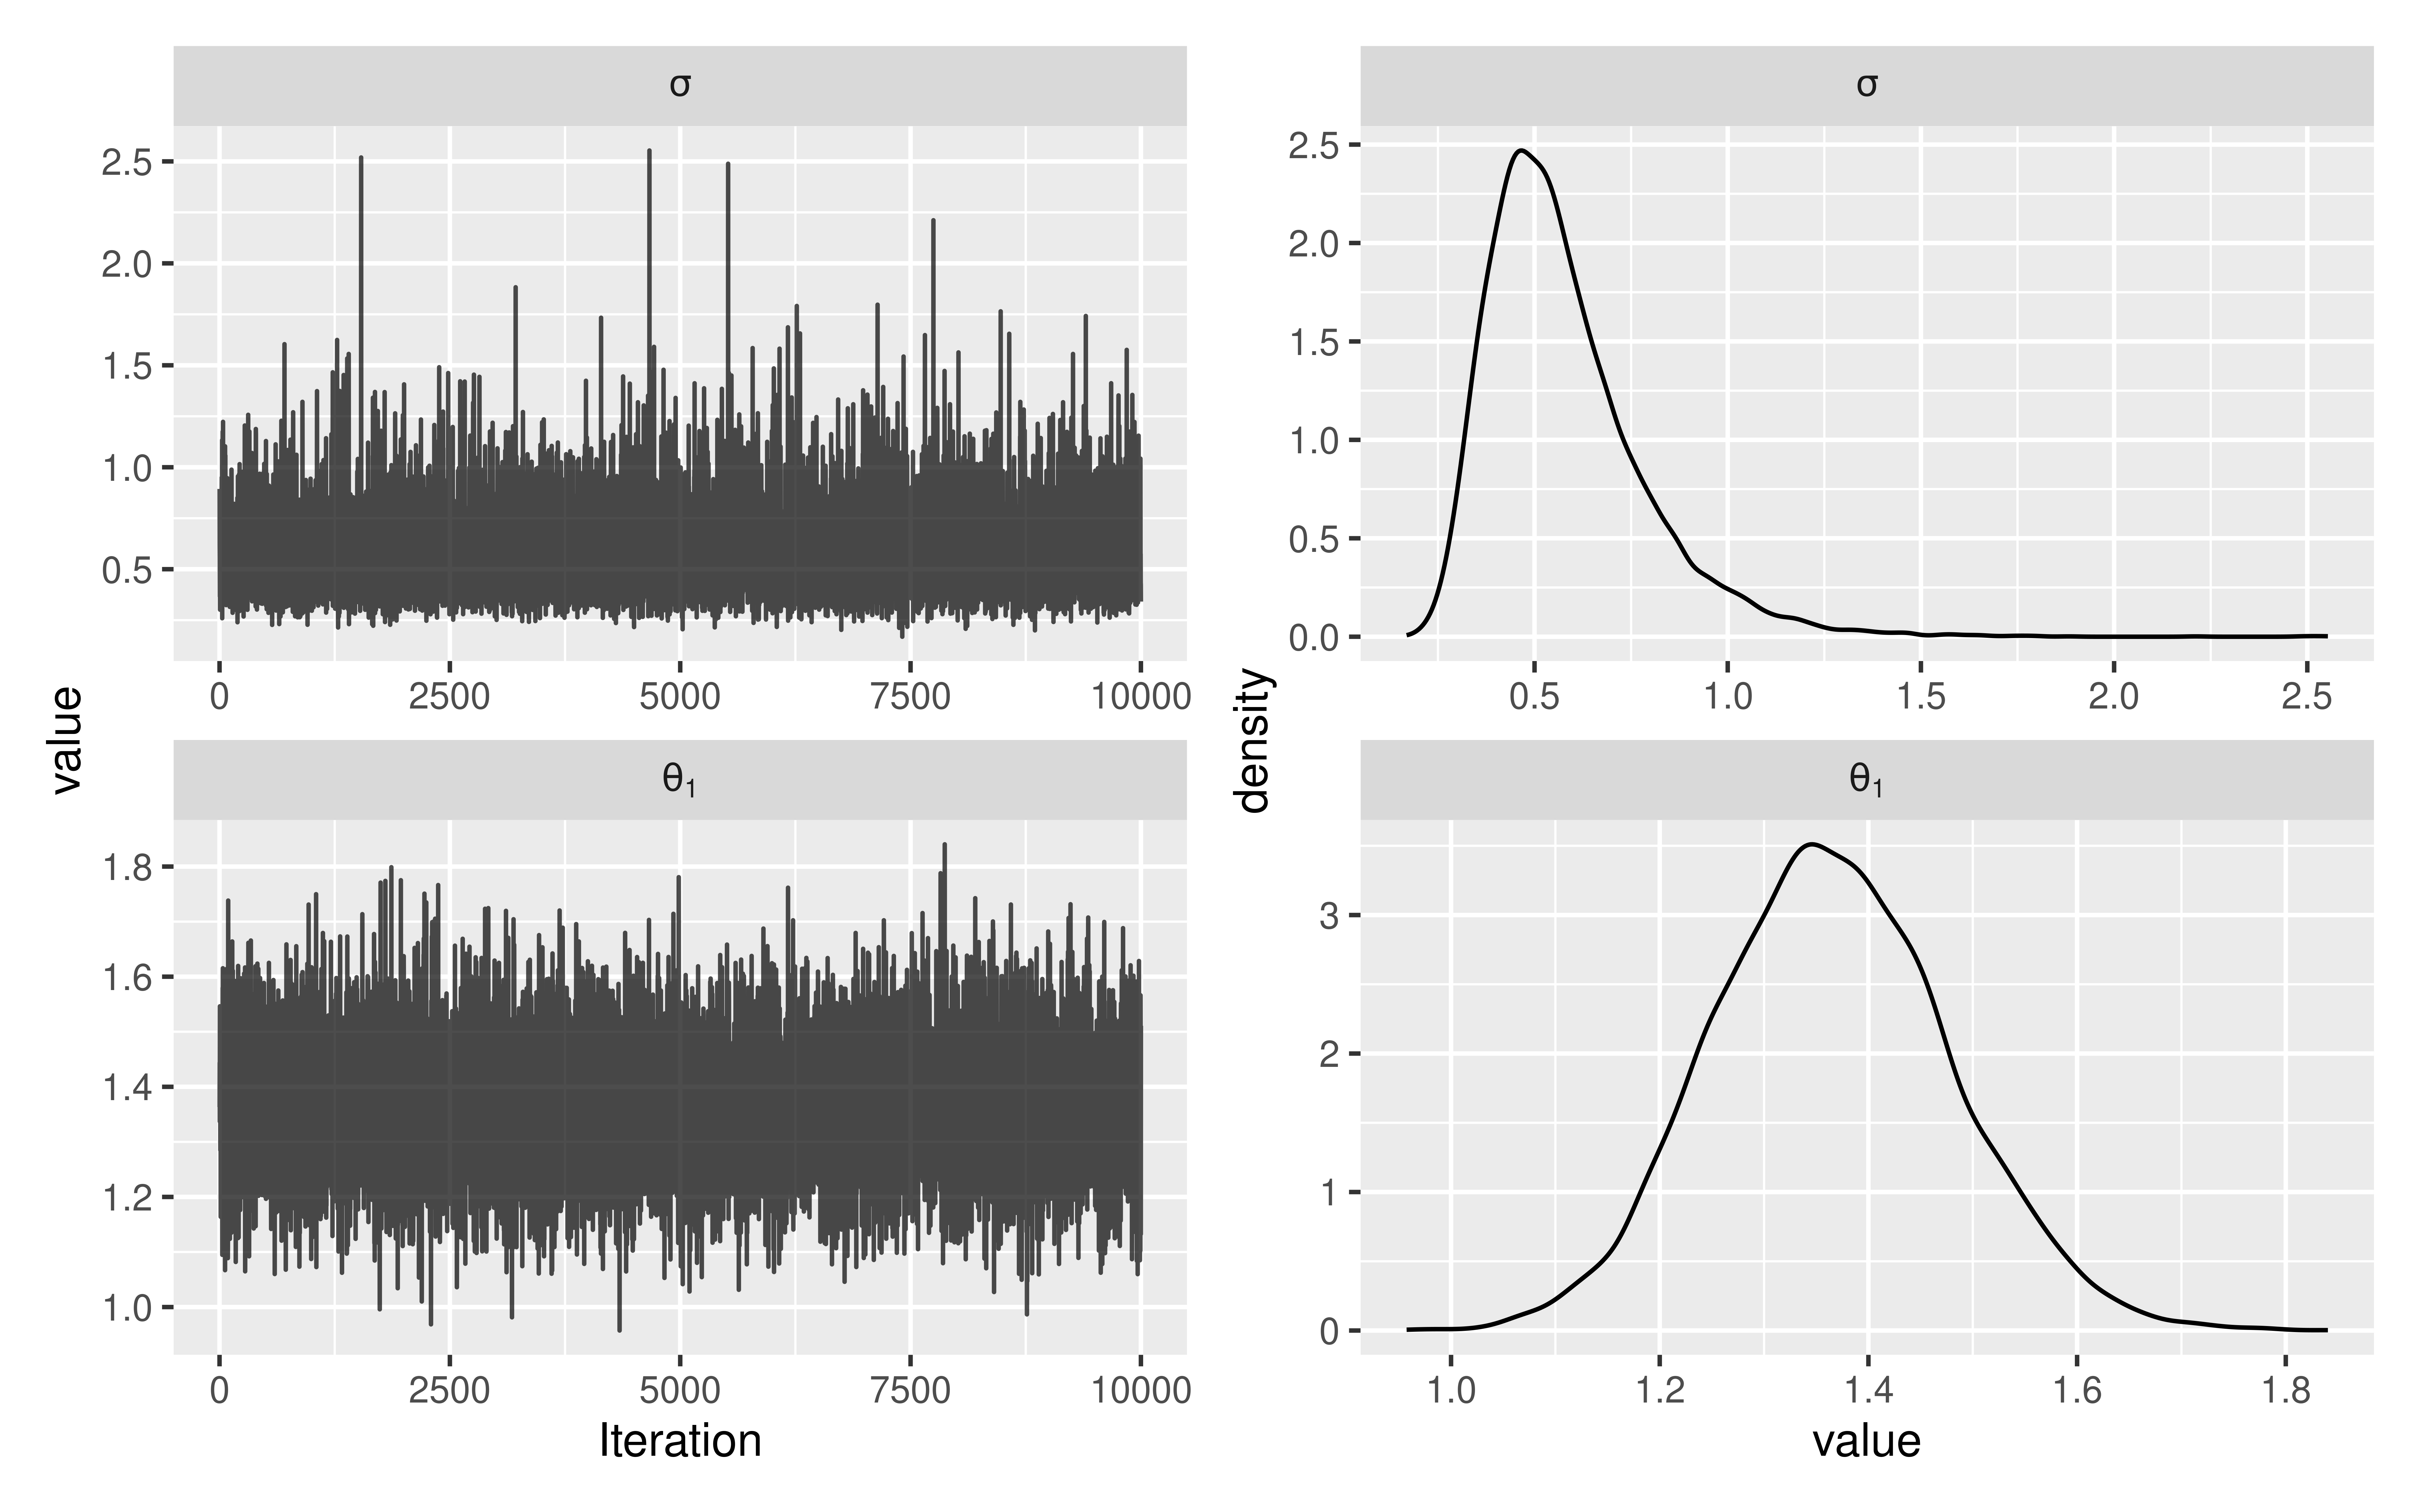
\includegraphics[width=\linewidth]{Images/Gibbs traceplot.png}}
    \caption{Апостеріорний розподіл параметрів~$\sigma$ та $\theta_1$ (засоби \texttt{R-base})}
    \label{pic: Gibbs Sampler traceplot}
\end{figure}

\vspace{0.4cm}
\begin{figure}[H]\centering
    \center{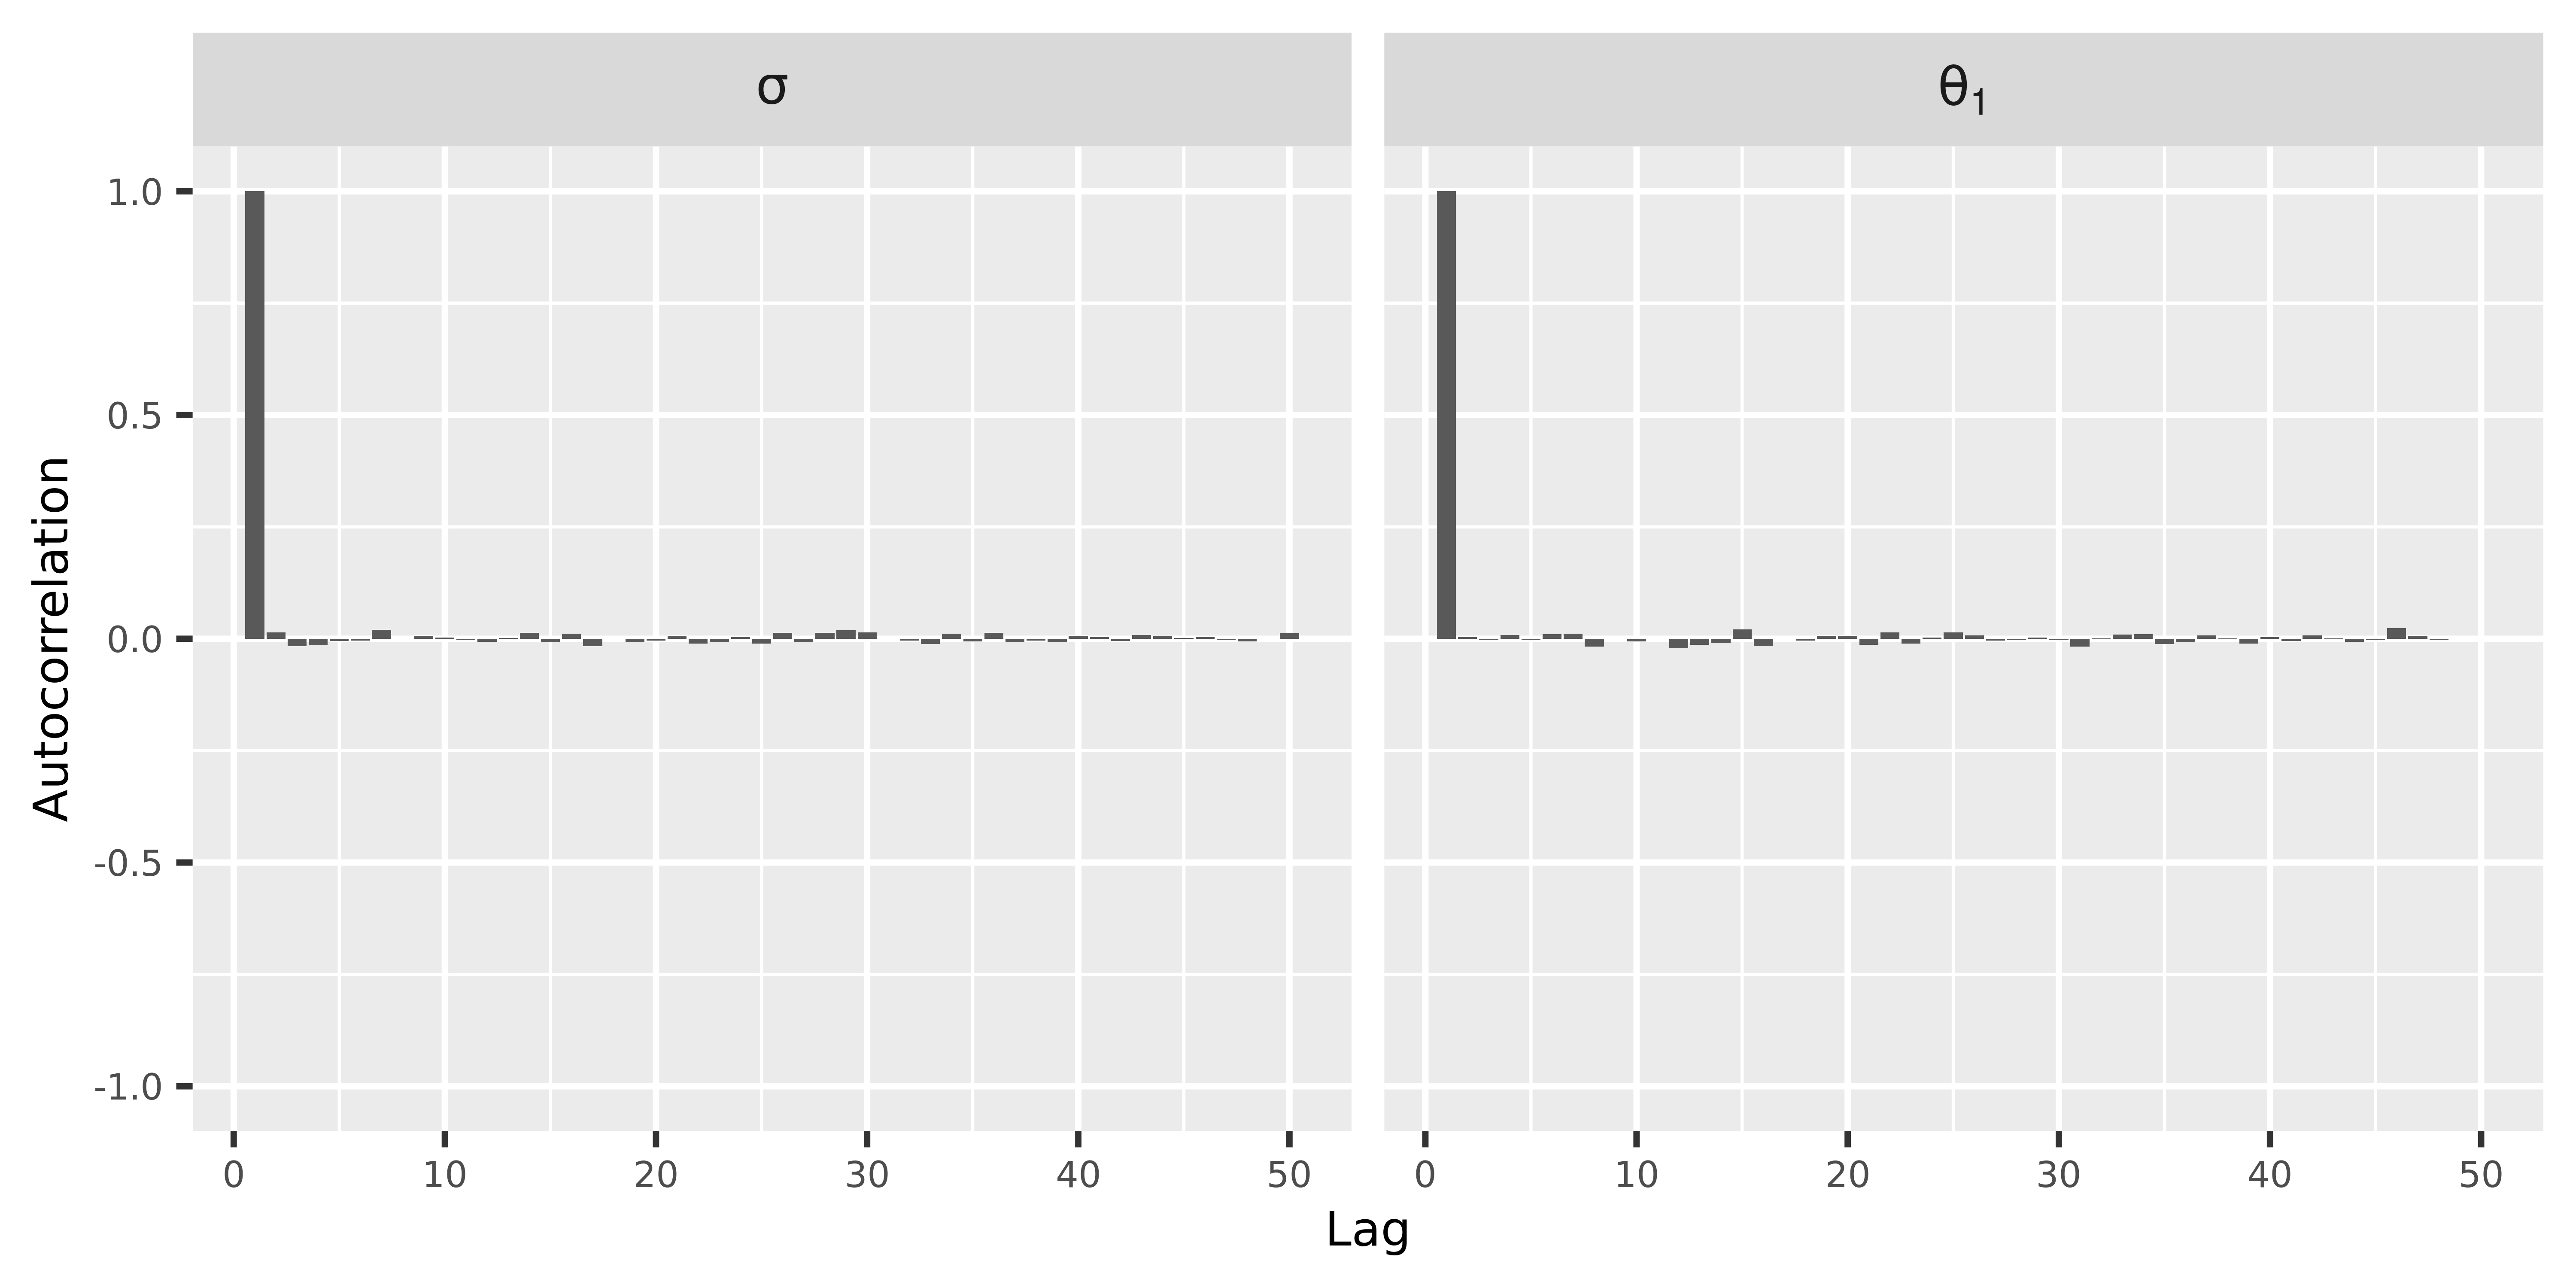
\includegraphics[width=\linewidth]{Images/Gibbs autocorrelation.png}}
    \caption{Автокореляційний графік параметрів~$\sigma$ та $\theta_1$ (засоби \texttt{R-base})}
    \label{pic: Gibbs Sampler autocorrelation}
\end{figure}

Аналогічні висновки про слабку колеляцію можна зробити із табличного вигляду автоколеляційного графіка (Табл.~\ref{table: Gibbs Sampler autocorrelation}).

\vspace{0.4cm}
\begin{table}[H]\centering
    \begin{tblr}{
            hlines={1pt,solid}, 
            vlines={1pt,solid},
            % hline{4-6}={1-5}{0pt},
            colspec={Q[3cm,c]Q[3cm,c]Q[3cm,c]},
            % cell{1}{1}={r=2,c=1}{c},
            % cell{1}{2}={r=1,c=2}{c},
            % cell{1}{4}={r=1,c=2}{c},
            column{2-3}={mode=math},
        }

               & \sigma   &  \theta_1 \\
        Lag 0  &  1.0000  &  1.0000   \\
        Lag 1  &  0.0141  &  0.0038   \\
        Lag 5  & -0.0036  &  0.0099   \\
        Lag 10 & -0.0027  & -0.0009   \\
        Lag 50 & -0.0018  &  0.0036   \\

    \end{tblr}
    \caption{Автокореляційна таблиця параметрів~$\sigma$ та $\theta_1$}
    \label{table: Gibbs Sampler autocorrelation}
\end{table}

У випадку ж сильної автокореляції значень у пригоді може стати виявлення так званого ефективного розміру вибірки (effective size), який вказуватиме, скільки значень у ланцюзі безпочередньо містять інформацію про стаціонарний розподіл. До прикладу, якщо згенеровано ланцюг довжиною~$N=10\,000$, а ефективний розмір вибірки складає~$N_{e.s.}=1000$, то це означає, що при обчисленні статистичних оцінок про істинний стаціонарний розподіл кожне~$N/N_{e.s.} = 100$-те значення містить цінну інформацію, а інші значення є високо корельованими.

\newpage
Для ланцюга, отриманого на Рис.~\ref{pic: Gibbs Sampler traceplot}, $N^{\sigma}_{e.s.} = N^{\theta_1}_{e.s.}=10\,000$, що при довжині ланцюга~$N=10\,000$ зайвий раз підкреслює відсутність автоколеляції, адже кожне значення містить корисну інформацію про стаціонарний розподіл.

Таким чином, наостанок наведемо деякі статистичні характеристики отриманих апостеріорних розподілів з точністю до чотирьох значущих знаків (Табл.~\ref{table: R-base Gibbs Sampler results}), зокрема вкажемо значення <<класичної>> Баєсової оцінки як умовного математичного сподівання.

\vspace{0.4cm}
\begin{table}[H]\centering
    \begin{tblr}{
            hlines={1pt,solid}, 
            vlines={1pt,solid},
            % hline{4-6}={1-5}{0pt},
            colspec={X[c]X[c]X[c]X[c]X[c]X[c]},
            % cell{1}{1}={r=2,c=1}{c},
            % cell{1}{2}={r=1,c=2}{c},
            % cell{1}{4}={r=1,c=2}{c},
            row{1}={m},
            row{2-3}={mode=math},
        }

        Parameter & Empirical mean & Standard deviation & Standard error & $2.5\%$ - quantile & $97.5\%$ - quantile \\
        \sigma    & 0.5768 & 0.2054 & 0.002054 & 0.3002 & 1.0800 \\
        \theta_1  & 1.3640 & 0.1139 & 0.001139 & 1.1478 & 1.5930 \\

    \end{tblr}
    \caption{Результати імплементації вибірки Гіббса засобами \texttt{R-base}}
    \label{table: R-base Gibbs Sampler results}
\end{table}

У задачах статистичного аналізу для оцінки невідомого параметра імовірнісної моделі використовують не лише точкові, але й інтервальні оцінки. При цьому, у так званому частотному підході такою оцінкою слугує довірчий інтервал (confidence interval), а у Баєсівському підході~--- імовірний інтервал (credible interval). У декількох наступних абзацах коротко наведемо відмінності між цими поняттями.

Нехай задано вибірку~$X_1,\ldots,X_n$ з деякого розподілу $f(x;\mu)$, де невідомим параметром слугує~$\mu$. У частотному підході значення~$\mu$ вважається невідомим та фіксованим. У ролі точкової оцінки може бути використана довільна статистика (скажімо, вибіркове середнє), і окремим питанням стоятиме визначення властивостей такої оцінки (змістовність, незміщеність тощо). Водночас, судження щодо значень параметра~$\mu$ можна зробити на основі довірчого інтервалу зі статистик~$T_1(\vv{X})$ та~$T_2(\vv{X}):$ 
\begin{equation}\label{eq: confidence interval}
    P(T_1(\vv{X}) < \mu < T_2(\vv{X})) \geq \gamma
\end{equation}

Інтервал~\eqref{eq: confidence interval} називають довірчим інтервалом рівня довіри~$\gamma$. Отриманий інтервал є випадковим проміжком, який слід трактувати так: серед (нескінченних) спроб побудувати довірчий інтервал~$\bigl( T_1(\vv{x}),T_2(\vv{x}) \bigr)$ для щоразу іншої реалізації вибірки~$\vv{x}$, щонайменше $\gamma\%$ з побудованих інтервалів міститимуть істинне значення невідомого параметра~$\gamma$. Тобто для конкретного наявного набору даних~$\vv{x}$ побудований інтервал або містить, або не містить істинний параметр. Іншими словами, значення~$\gamma$ має не імовірнісну інтерпретацію наявності/відсутності істинного значення параметра у побудованому довірчому інтервалі, а радше <<рівнем впевненості>> безпосередньо у статистичній процедурі побудови інтервалу.

На противагу частотному підходу, Баєсівська модель вважає параметр~$\mu$ невідомою випадковою величиною. Відтак, шляхом переоцінки деякого апріорного розподілу~$\mu \sim g(x)$ із залученням конкретного набору даних~$\vv{x}$, судження про значення параметра виконують з отриманого переоціненого апостеріорного розподілу~$g^{*}(x)$. Подальшим кроком може бути побудова точкої оцінки чи визначення імовірного інтервалу
\begin{equation}\label{eq: credible interval}
    P(q_1 < \mu < q_2) \overset{\scalebox{0.5}{def}}{=} \int\limits_{q_1}^{q_2} g^{*}(x)\, dx,
\end{equation}
який означатиме, власне, імовірність параметра~$\mu$ належати проміжку~$(q_1,q_2)$ при наявних даних~$\vv{x}$. 

Отже, повертаючись до Баєсової моделі~\eqref{task 5 - eq: Bayes model Xij} -- \eqref{task 5 - eq: Bayes model sigma}, з огляду на результати побудованих апостеріорних розподілів (Табл.~\ref{table: R-base Gibbs Sampler results}), $95\%$-імовірний інтервал для значень параметра~$\theta_1$ матиме вигляд:
\begin{equation}\label{eq: theta1 R-base credible interval}
    P(1.1478 < \theta_1 < 1.5930) = 0.95
\end{equation}

Крім того, згідно вимог завдання порівняємо наведене значення зі значенням оцінки~\eqref{eq: my BE}, отриманої в рамках Завдання 4:
\begin{equation}\label{eq: R-base theta star estimation}
    \widehat{\theta}_1 = \left( k/m+\overline{X}_1 \right)\left( \frac{\overline{X}}{k/m+\overline{X}} \right) = 1.3608
\end{equation}

\subsubsection*{Завдання (c): \texttt{R-jags} Gibbs Sampler}
\addcontentsline{toc}{subsection}{Завдання (c): \texttt{R-jags} Gibbs Sampler}

Тепер скористаємося засобами мови \texttt{R}, пакетом \texttt{rjags}, для реалізації вибірки Гіббса. Вибірку даних~\eqref{task 5 - eq: Bayes model Xij} задамо з файлу \texttt{hw5.csv}. Покладемо~$n=k=3$ та $m=100$, тобто матимемо Баєсову модель вигляду
\begin{align}
    & X_{ij} \,|\, \theta_i \overset{\scalebox{0.5}{ind}}{\sim} \mathrm{Poiss}(\theta_i),\ i=\overline{1,3},\ j=\overline{1,100}, \\
    & \theta_i \,|\, \sigma \overset{\scalebox{0.5}{i.i.d.}}{\sim} \mathrm{Gamma}(3,\sigma),\ i=\overline{1,3}, \\
    & \sigma^{-1} \sim \mathrm{Exp}(1)
\end{align}

Перш ніж рухатися далі, наголосимо, що параметр~$\sigma$ у Гамма-розподілі є <<scale parameter>>, в той час як засаби \texttt{rjags} надають можливість задати модель виключно через <<rate parameter>>. У такому разі, еквівалентний запис моделі матиме вид:
\begin{align}
    & X_{ij} \,|\, \theta_i \overset{\scalebox{0.5}{ind}}{\sim} \mathrm{Poiss}(\theta_i),\ i=\overline{1,3},\ j=\overline{1,100}, \\
    & \theta_i \,|\, \sigma \overset{\scalebox{0.5}{i.i.d.}}{\sim} \mathrm{Gamma}(3,\sigma^{-1}),\ i=\overline{1,3}, \\
    & \sigma^{-1} \sim \mathrm{Exp}(1)
\end{align}

Відтак, запис моделі через синтаксис \texttt{rjags} наведено на Лістингу~\ref{code: jags gibbs sampler}, а безпосередній запуск алгоритму вказано у Лістингу~\ref{code: run jags gibbs sampler}.

\vspace{0.4cm}
\begin{lstlisting}[
    style           = myR, 
    % backgroundcolor = {},
    caption         = {Задана модель засобами \texttt{rjags}},
    label           = {code: jags gibbs sampler},
]
jags_model_string <- "model {
    for (i in 1:(n*m)) {
        x[i] ~ dpois(theta[group[i]])
    }

    for (j in 1:n) {
        theta[j] ~ dgamma(k, invsigma)
    }

    invsigma ~ dexp(1.0)
}"
\end{lstlisting}

\vspace{0.4cm}
\begin{lstlisting}[
    style           = myR, 
    % backgroundcolor = {},
    caption         = {Запуск вибірки Гіббса засобами \texttt{rjags}},
    label           = {code: run jags gibbs sampler},
]
# Convert three flows of data (x1,x2,x3) into one list and label each datapoint accordingly (group 1.0, 2.0 or 3.0)
x_jags <- array(dim = c(m * n, 2))
colnames(x_jags) <- c("x", "group")

x_jags[1:100, 1] <- x[, 1]
x_jags[1:100, 2] <- 1.0

x_jags[101:200, 1] <- x[, 2]
x_jags[101:200, 2] <- 2.0

x_jags[201:300, 1] <- x[, 3]
x_jags[201:300, 2] <- 3.0

data_jags <- list(
    x = x_jags[, 1],
    group = x_jags[, 2],
    n = n,
    m = m,
    k = prior$k
)

model <- jags.model(
    textConnection(jags_model_string),
    data = data_jags,
    n.chains = 3,
)

update(model, 100) # burn-in period

params <- c("theta", "invsigma")

model_simulation <- coda.samples(
    model = model,
    variable.names = params,
    n.iter = 10e3
)
\end{lstlisting}

\vspace{0.4cm}

\newpage
В рамках додаткового дослідження збіжності МСМС було запущено три ланцюги з різних початкових точок відліку. У першому наближенні з Рис.~\ref{pic: jags Gibbs Sampler traceplot} можна зробити висновок, що бажана збіжність досягнута. 

\vspace{0.4cm}
\begin{figure}[H]\centering
    \center{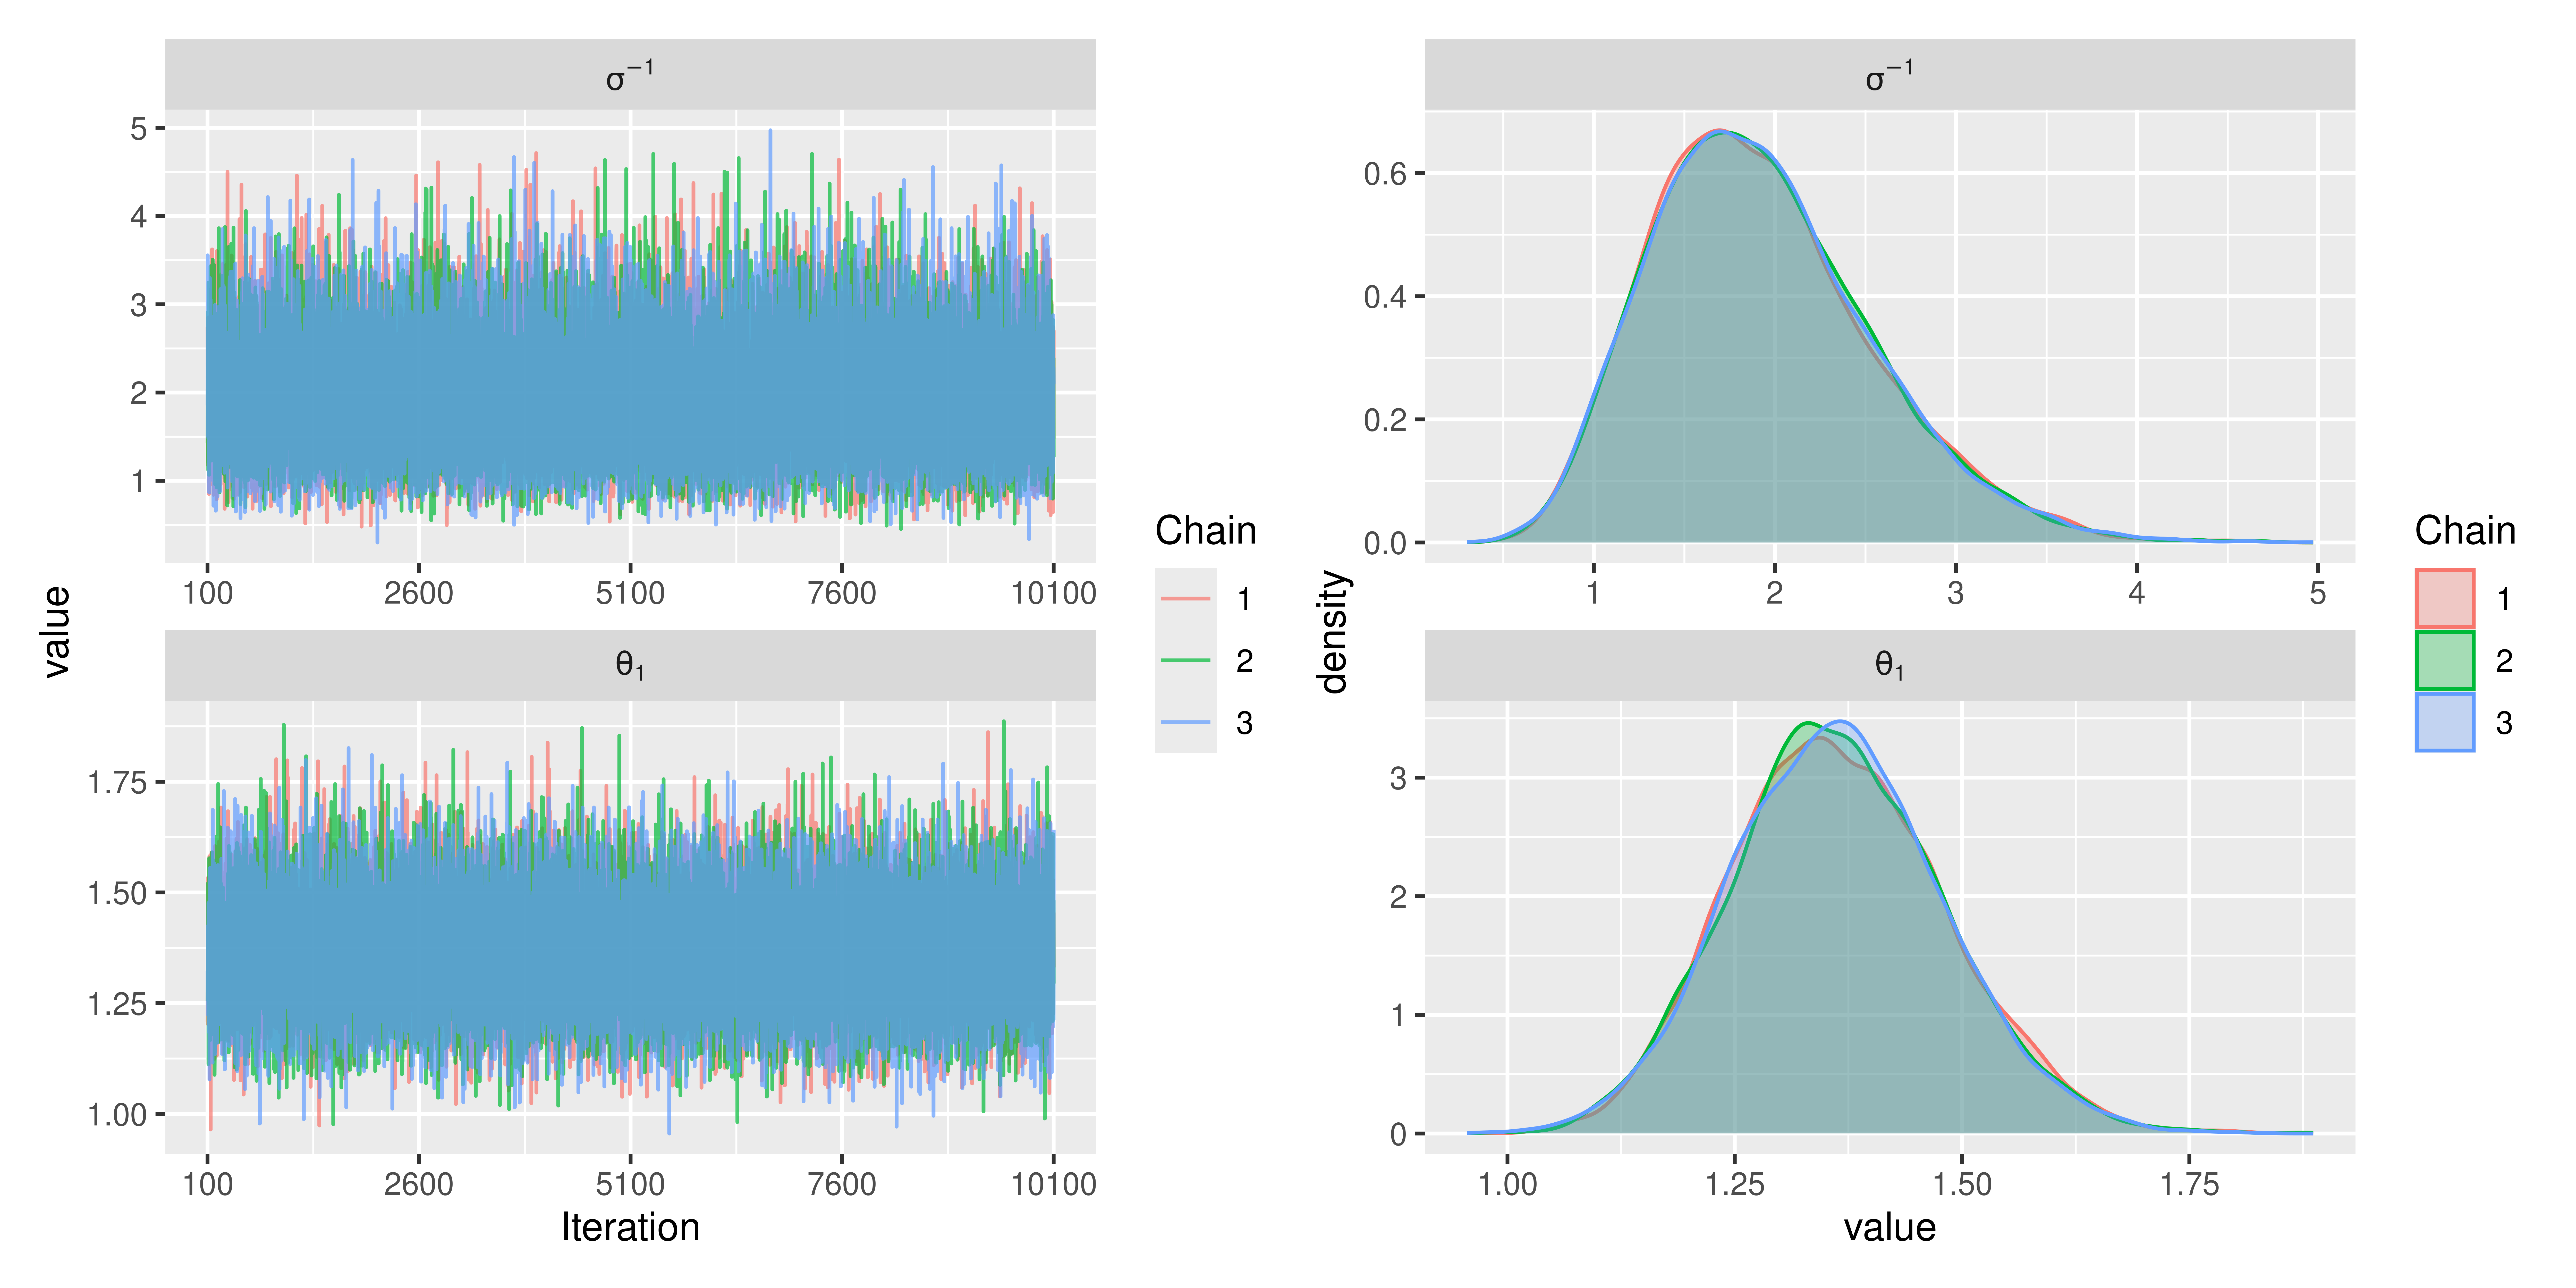
\includegraphics[width=\linewidth]{Images/JAGS Gibbs traceplot.png}}
    \caption{Апостеріорний розподіл параметрів~$\sigma^{-1}$ та $\theta_1$ (засоби \texttt{R-jags})}
    \label{pic: jags Gibbs Sampler traceplot}
\end{figure}

Тим не менш, додатковим кроком проведемо діагностику Гелмана-Рубіна (Gelman-Rubin diagnostic), яка полягає у визначенні своєрідної міри розрізненості між декількома ланцюгами. Діагностика обчислює варіабельність (розкид, дисперсію) всередині ланцюгів, порівнюючи її з дисперсією між ланцюгами. Якщо всі ланцюги наблизилися до стаціонарного розподілу, то варіабельність між ланцюгами має бути відносно невеликою, а так званий <<коефіцієнт потенційного зменшення масштабу>> (potential scale reduction factor), який є результатом діагностики, має бути близьким до одиниці. Якщо значення значно перевищує одиницю, то можна зробити висновок, що ланцюги ще не збіглися за задану кількість ітерацій.

Бачимо (Рис.~\ref{pic: jags Gibbs Sampler gelman diagnostic}), що значення конфіцієнта близьке до одиниці як для параметра~$\sigma$, так і для параметра~$\theta_1$. Більш того, спостерігаємо, що бажана збіжність досягнута вже на початкових ітераціях, тому <<період розгону>> ланцюга (burn-in period) було обачно покласти невеликим: 100 перших ітерацій (Лістинг~\ref{code: run jags gibbs sampler}).

\vspace{0.4cm}
\begin{figure}[H]\centering
    \center{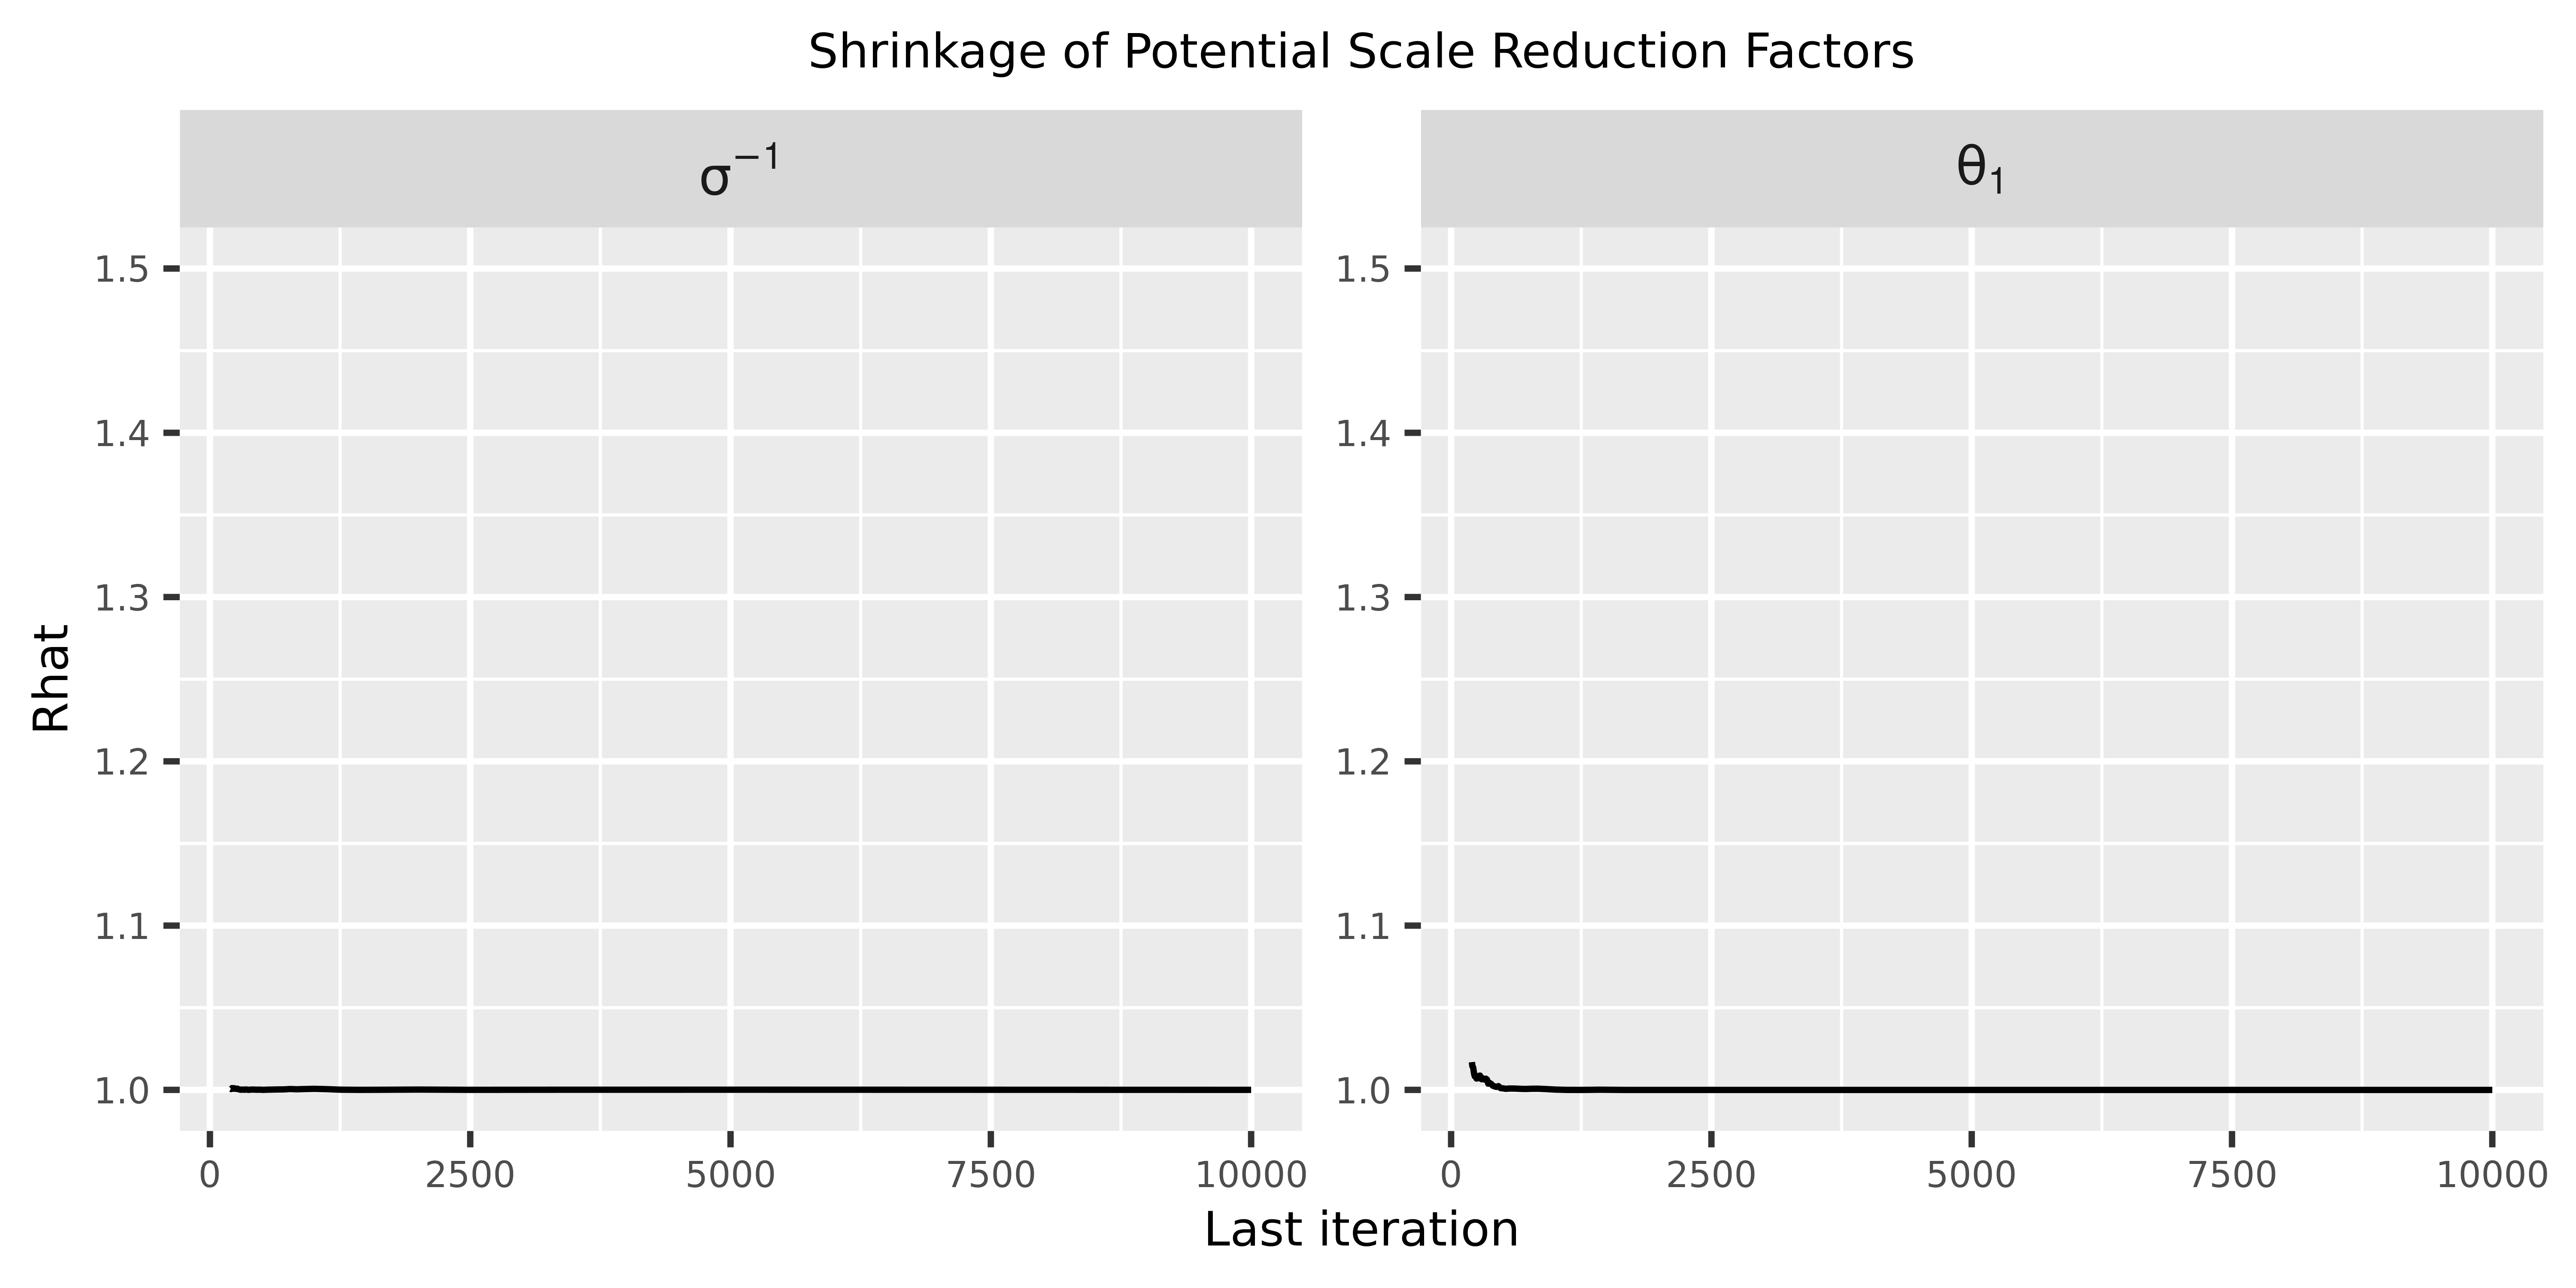
\includegraphics[width=\linewidth]{Images/JAGS Gibbs gelman diagnostic.png}}
    \caption{Діагностика Гелмана-Рубіна для параметрів~$\sigma^{-1}$ та $\theta_1$}
    \label{pic: jags Gibbs Sampler gelman diagnostic}
\end{figure}

Таким чином, у підсумку розглянемо перший з трьох ланцюгів, для якого дослідимо ознаки автокореляції (Рис.~\ref{pic: jags Gibbs Sampler autocorrelation}) та побудуємо Баєсівські оцінки (Табл.~\ref{table: R-jags Gibbs Sampler results}), які можна вважати змістовними та нідійними, адже ефективний розмір вибірки (effective size) при довжині ланцюга~$N=10\,000$ є значним:~$N^{\sigma^{-1}}_{e.s.} = N^{\theta_1}_{e.s.} = 10\,000$.

\vspace{0.4cm}
\begin{figure}[H]\centering
    \center{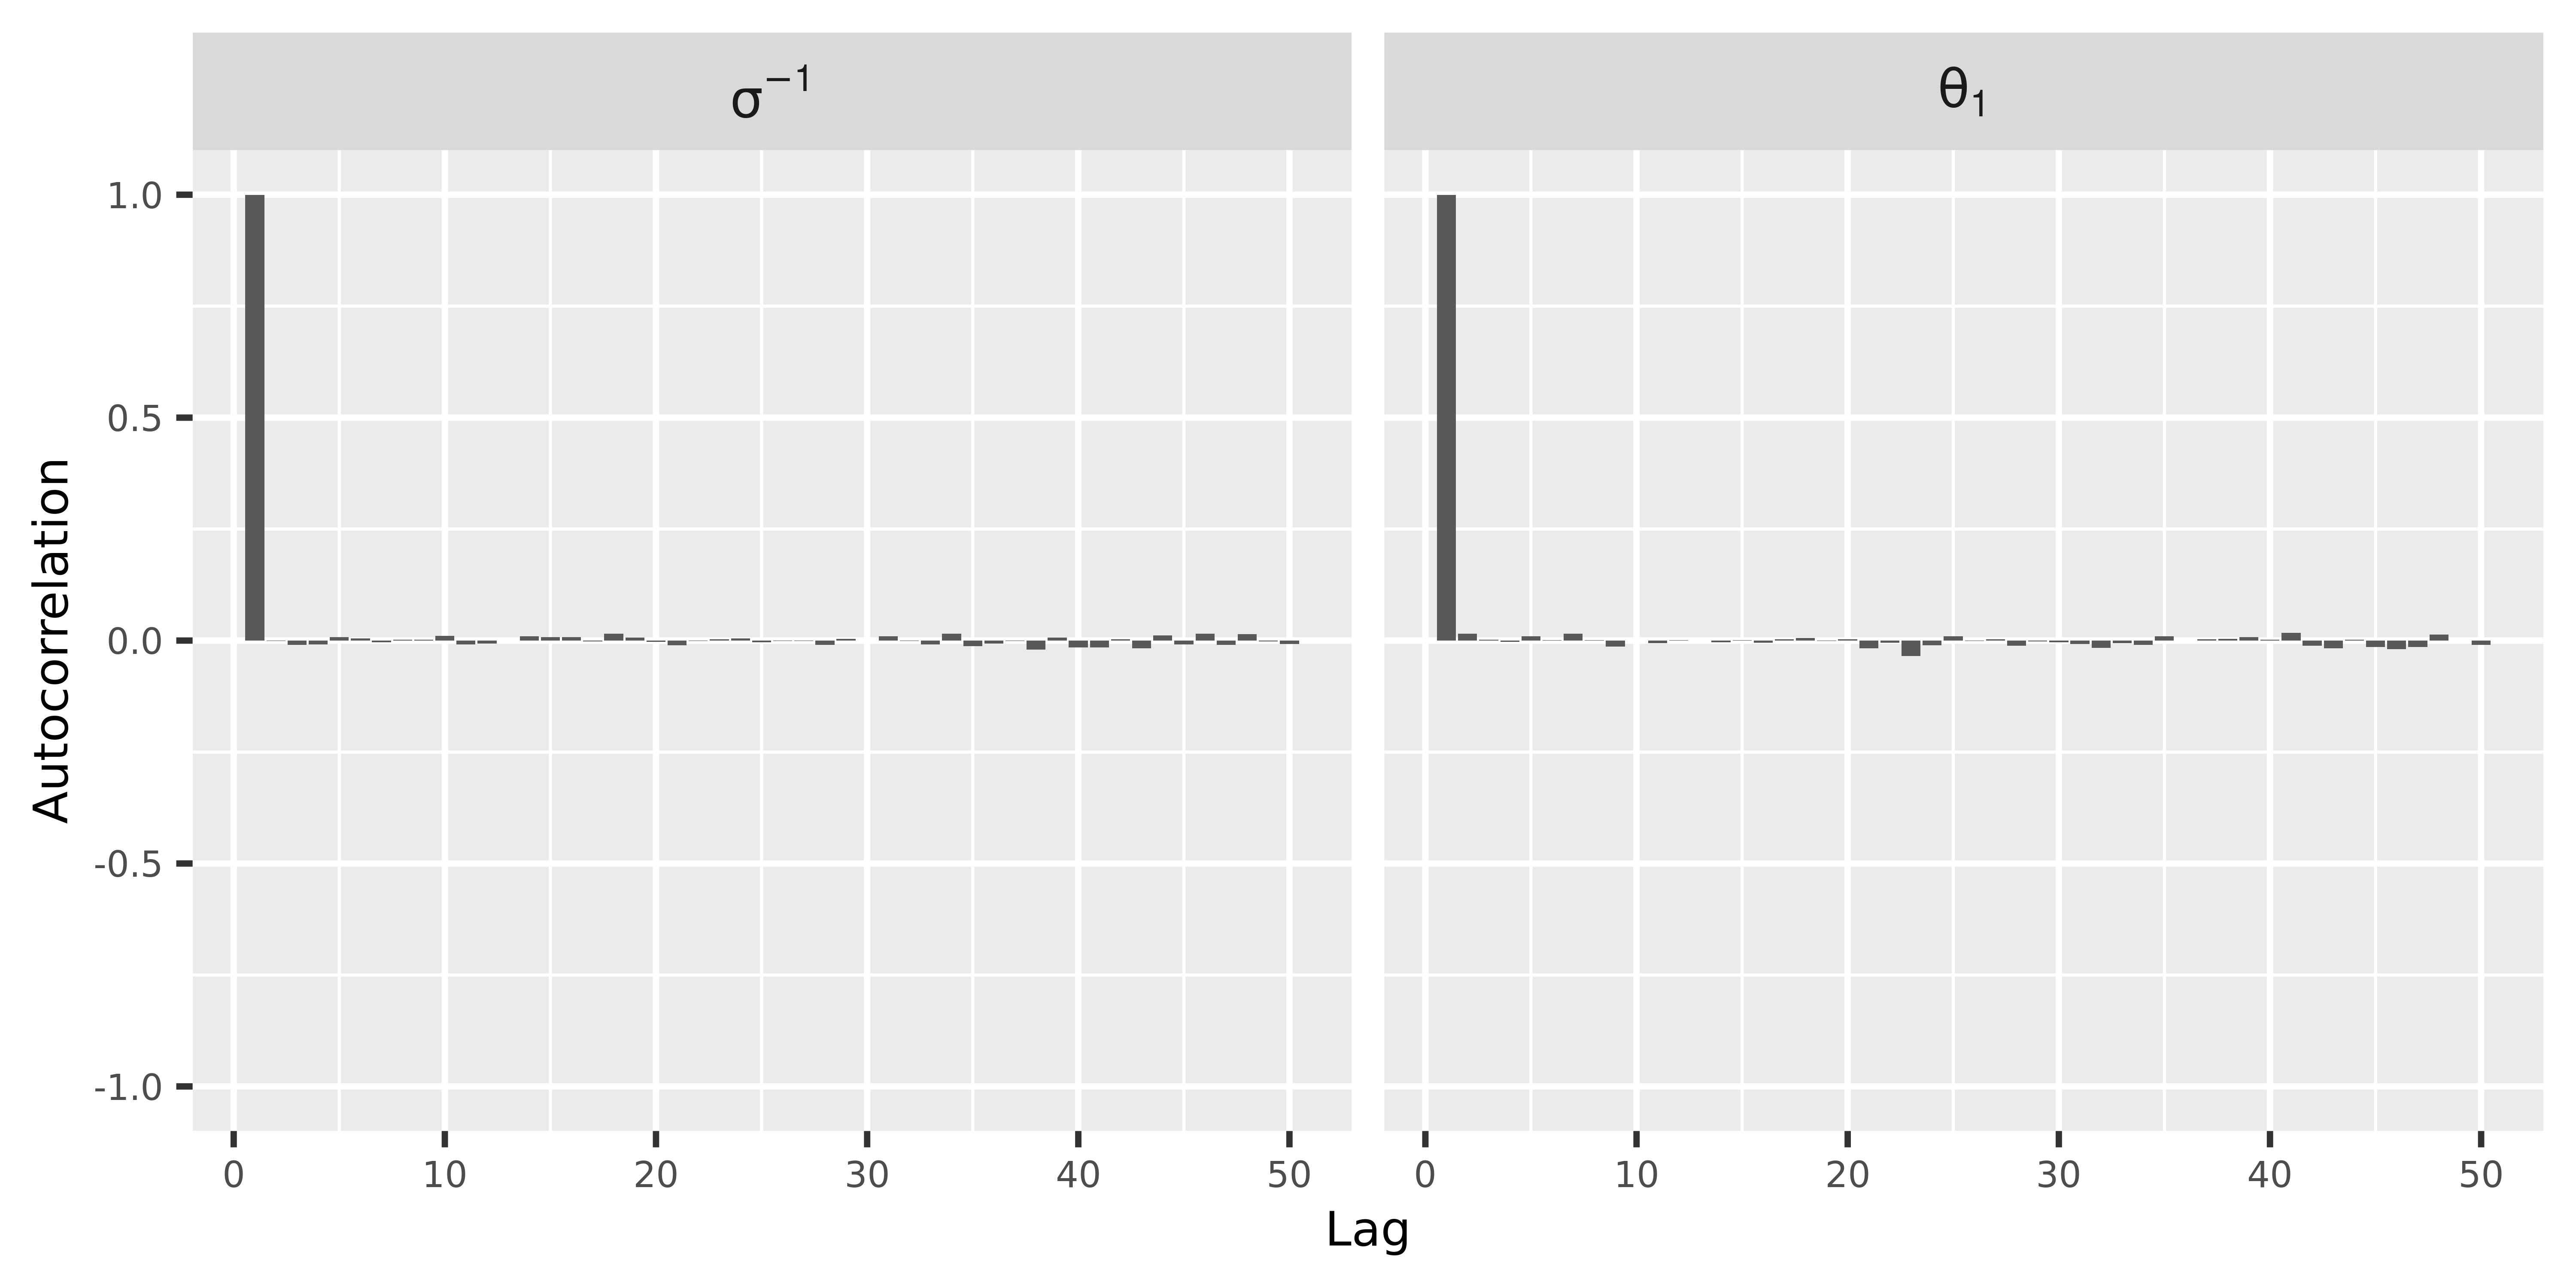
\includegraphics[width=\linewidth]{Images/JAGS Gibbs autocorrelation.png}}
    \caption{Автокореляційний графік параметрів~$\sigma^{-1}$ та $\theta_1$ (засоби \texttt{R-jags})}
    \label{pic: jags Gibbs Sampler autocorrelation}
\end{figure}

\vspace{0.4cm}
\begin{table}[H]\centering
    \begin{tblr}{
            hlines={1pt,solid}, 
            vlines={1pt,solid},
            % hline{4-6}={1-5}{0pt},
            colspec={X[c]X[c]X[c]X[c]X[c]X[c]},
            % cell{1}{1}={r=2,c=1}{c},
            % cell{1}{2}={r=1,c=2}{c},
            % cell{1}{4}={r=1,c=2}{c},
            row{1}={m},
            row{2-3}={mode=math},
        }

        Parameter & Empirical mean & Standard deviation & Standard error & $2.5\%$ - quantile & $97.5\%$ - quantile \\
        \sigma^{-1} & 0.9210 & 0.6130 & 0.006130 & 0.9131 & 1.2990 \\
        \theta_1    & 1.3640 & 0.1153 & 0.001153 & 1.1458 & 1.5970 \\

    \end{tblr}
    \caption{Результати імплементації вибірки Гіббса засобами \texttt{R-jags}}
    \label{table: R-jags Gibbs Sampler results}
\end{table}

Наостанок, $95\%$-імовірний інтервал для значень параметра~$\theta_1$ матиме вигляд:
\begin{equation}\label{eq: theta1 R-jags credible interval}
    P(1.1458 < \theta_1 < 1.5970) = 0.95,
\end{equation}
що практично повторює отримані результати~\eqref{eq: theta1 R-base credible interval}. Водночас, значення оцінки~\eqref{eq: my BE}, отриманої в рамках Завдання 4, є таким:
\begin{equation}\label{eq: R-jags theta star estimation}
    \widehat{\theta}_1 = \left( k/m+\overline{X}_1 \right)\left( \frac{\overline{X}}{k/m+\overline{X}} \right) = 1.3608
\end{equation}